%----------------------------------------------------------------------------------------
% NKUST EC Master Thesis
% Original authors : AIoRLab/NCLab/WNDCLab Thesis LaTeX Team
% Department of Electronic Engineering
% National Kaohsiung University of Sciences and Technology
% GitHub : https://github.com/yuhao-kuo/NKUST-thesis-template
% Version 1.0 (2020.01.31)
%----------------------------------------------------------------------------------------

%----------------------------------------------------------------------------------------
%	PACKAGES AND OTHER DOCUMENT CONFIGURATIONS
%----------------------------------------------------------------------------------------

\documentclass[oneside,
12pt, % The default document font size, options: 10pt, 11pt, 12pt
%oneside, % Two side (alternating margins) for binding by default, uncomment to switch to one side
english, % ngerman for German
onehalfspacing, % Single line spacing, alternatives: onehalfspacing or doublespacing
%draft, % Uncomment to enable draft mode (no pictures, no links, overfull hboxes indicated)
%nolistspacing, % If the document is onehalfspacing or doublespacing, uncomment this to set spacing in lists to single
%liststotoc, % Uncomment to add the list of figures/tables/etc to the table of contents
%toctotoc, % Uncomment to add the main table of contents to the table of contents
%parskip, % Uncomment to add space between paragraphs
]{NKUSThesis} % The class file specifying the document structure

% ----- 論文資訊 -----
% ------------ 作者資訊 ------------

% 註: 下文中如有 en 表示為英文資訊,標注 tw 表示為正體中文資訊。

% 研究生名字
\def\authortwname{王小明}
\def\authorenname{Shio-Min Wang}

% 指導教授名字
\def\supervisortwname{孫思邈 博士}
\def\supervisorenname{Si-Miao Sun Ph.D.}
% 共同指導教授名字
\def\cosupervisortwname{李時珍 博士}
\def\cosupervisorenname{Shi-Zhen Li Ph.D.}

% 學校
\def\schooltwname{國立高雄科技大學}
\def\schoolenname{National Kaohsiung University of Science and Technology}
% 地區
\def\schoolenlocation{Kaohsiung, Taiwan, Republic of China}
% 原合併前校區
\def\schoolenoldname{National Kaohsiung University of Applied Sciences} % 國立高雄科技大學由"國立高雄應用科技大學/國立高雄第一科技大學/國立高雄海洋科技大學"三所科技大學合併而成,此欄位請填入原先校區所屬學校英文名稱。

% 主修項目
\def\majortwname{Electronic Engineering}
% 系所名稱
\def\depttwname{電子工程系}
\def\deptenname{Department of Electronic Engineering}

% 學位
\def\degreetw{碩士}
\def\degreeen{Master}

% 論文題目
\def\titletw{高雄科技大學LaTeX論文樣板}
\def\titleen{NKUST LaTeX Thesis Template}

% 日期(月份)
\def\dateROC{中華民國 一一一 年 六 月}
\def\dateen{Jun, 2022}

% pdf search keywords
\def\thesiskeywords{{LaTeX},{NKUST},{Thesis},{Template}}


% ----- 版型設定 -----


\setcounter{secnumdepth}{6}
\setcounter{tocdepth}{6}

% ----------------------------
%   文字字型設定
% ----------------------------

% xelatex 中文套件設定
\usepackage[SlantFont]{xeCJK} % 中文字體支援(xelatex)
\usepackage[LGR,OT1]{fontenc} % Output font encoding for international characters
\usepackage{palatino} % Use the Palatino font by default
\usepackage{indentfirst} \setlength{\parindent}{2em}
\usepackage{lipsum}
\usepackage{fontspec}
\usepackage[english]{babel} % 外國語系字母支援

\defaultfontfeatures{AutoFakeBold=2.5,AutoFakeSlant=.2}

% 英文字體設定(可自行更改)
\setmainfont[Path=./Fonts/]{DejaVuSerif}

% 英文字家族範例
\newcommand*{\edukai}{\CJKfamily{edukai-4.0}}
\renewcommand*{\rmdefault}{lmr}
\renewcommand*{\sfdefault}{lmss}
\renewcommand*{\ttdefault}{lmtt}

% 中文字體設定(教育部標準字體)
\setCJKmainfont[Path=./Fonts/]{edukai-4.0}
\setCJKmonofont[Path=./Fonts/]{edukai-4.0}
\setCJKsansfont[Path=./Fonts/]{edukai-4.0}

% ----------------------------
%   排版擴充
% ----------------------------
\newcommand\n{\mbox{\qquad}} % 換行指令
\usepackage{xcolor}	% 字體顏色
\usepackage{lettrine}  % 空白間距
\usepackage[autostyle=true]{csquotes} % 引號排版
\usepackage{indentfirst} % 首行縮排
\usepackage{setspace} % 行距
\usepackage{scrbase}
\usepackage{scrhack}
\usepackage{Templates/nkusthesis_layout} % 版面排版

% ----------------------------
%   排序
% ----------------------------
\usepackage{amsmath}

\numberwithin{figure}{section}

\newtheorem{definition}{Definition}
\newtheorem{problem}{Problem}

\newtheorem{theorem}{Theorem}[section]
\newtheorem{lemma}[theorem]{Lemma}
\newtheorem{note}[theorem]{Note}
\newtheorem{corollary}[theorem]{Corollary}
\newtheorem{prop}[theorem]{Proposition}

\newtheorem{thm}{Theorem}%[section]
\newtheorem{lma}{Lemma}%[theorem]
\newtheorem{defi}{Definition}
\newtheorem{rul}{Rule}

% ----------------------------
%   章節
% ----------------------------
\usepackage{titlesec}
\usepackage{titletoc}
\usepackage{zhnumber}
\usepackage{CJKnumb}	% 阿拉伯數字轉中文字

% ----------------------------
%   超連結
% ----------------------------
\usepackage{hyperref}
\usepackage{url}

\hypersetup{pdfpagemode={UseOutlines},
	linktocpage,		% 
	bookmarksopen=true,
	bookmarksopenlevel=0,
	hypertexnames=false,
	colorlinks=true, % Set to false to disable coloring links
	citecolor=red, % The color of citations
	linkcolor=blue, % The color of references to document elements (sections, figures, etc)
	urlcolor=magenta, % The color of hyperlinks (URLs)
	pdfstartview={FitV},
	unicode,
	breaklinks=true,
	pdfcreator={NKUST LaTeX Template Groups},
	pdfproducer={NKUST LaTeX template build on XeLaTeX},
	pdftitle={\titletw\ \titleen},						% 文件標題
	pdfsubject={\authorenname, \degreeen\ thesis - \titleen},	% 文件主旨
	pdfauthor={\authorenname \ \authortwname},					% 擁有者
	pdfkeywords={\thesiskeywords},	% 關鍵字
}

\pdfstringdefDisableCommands{ % If there is an explicit linebreak in a section heading (or anything printed to the pdf-bookmarks), it is replaced by a space
	\let\\\space
}

% ----------------------------
%   內文排版
% ----------------------------

%   程式碼區塊
\usepackage{listings}
\usepackage{xcolor}

\definecolor{codegreen}{rgb}{0,0.6,0}
\definecolor{codegray}{rgb}{0.5,0.5,0.5}
\definecolor{codepurple}{rgb}{0.58,0,0.82}
\definecolor{backcolour}{rgb}{0.95,0.95,0.92}
\lstdefinestyle{codestyle}{
    backgroundcolor=\color{backcolour},   
    commentstyle=\color{codegreen},
    keywordstyle=\color{magenta},
    numberstyle=\tiny\color{codegray},
    stringstyle=\color{codepurple},
    basicstyle=\textrm\footnotesize,
    breakatwhitespace=false,         
    breaklines=true,                 
    captionpos=b,                    
    keepspaces=true,                 
    numbers=none,                    
    numbersep=5pt,                  
    showspaces=false,                
    showstringspaces=false,
    showtabs=false,                  
    tabsize=2
}

\lstset{style=codestyle}

%   演算法虛擬碼
\usepackage{algorithm}
\usepackage{algorithmicx}
\usepackage{algpseudocode}

%   小圖
\usepackage{subfigure}

%   原文顯示支援
\usepackage{verbatim}
\usepackage{moreverb}



%   表格
\usepackage{multirow}
\usepackage{makecell}
\usepackage{threeparttable}
\usepackage{longtable}
\usepackage{booktabs}

%   外部PDF導入
\usepackage{pdfpages}

% 曲線繪圖
\usepackage{tikz}

% 資料繪圖
\usepackage{pgfplots}
\usepgfplotslibrary{colorbrewer}
\pgfplotsset{compat=newest,compat/show suggested version=false}
\usepackage[subpreambles]{standalone}

% 繪圖
\usepackage{graphicx} % Required to include images
\graphicspath{{Figures/}{./}} % Specifies where to look for included images

% 流程狀態圖繪圖
\usepackage{amscd}

% 數學符號擴充
\usepackage{amssymb}

% 數學公式擴充
\usepackage{amsthm}

% 符號擴充
\usepackage{siunitx}

% 圖片
\usepackage{eso-pic}
\usepackage{picture}
\usepackage{wallpaper}

% 浮水印
\usepackage[contents=]{background} %如果沒有給 contest空白會自動加上 draft 浮水印字樣

% 浮水印參數定義
\newcommand\NTUSTwatermark {
	\backgroundsetup{
		contents={\includegraphics{\watermarkimage}},
		angle=0,
		opacity=0.2,
		hshift = 0mm,
		vshift = 0mm,
		scale=0.5
	}
}

% 章節
\usepackage{caption}
\captionsetup[centerlast,small,n]{name=caption} % setting caption
\setlength{\captionmargin}{50pt}

% ----------------------------
%   頁首頁尾
% ----------------------------
\usepackage[Lenny]{fncychap}
\pagestyle{empty}

% ----------------------------
%   其他擴充功能
% ----------------------------

%   if-else 擴充
\usepackage{ifthen}

%   variable checked
\usepackage{etoolbox}

% ----------------------------
%   其他定義
% ----------------------------

% Other
\newcommand{\checktoopen}{% New command to move content to the next page which prints to the next odd page if twosided mode is active
\if@openright\cleardoublepage\else\clearpage\fi
}

\newcommand\bhrule{\typeout{--------------------}}
\newcommand\tttypeout[1]{\bhrule\typeout{\space #1}\bhrule}

\newcommand{\HRule}{\rule{\linewidth}{0.5mm}} % New command to make the lines in the title page
\newcommand{\decoRule}{\rule{.8\textwidth}{.4pt}} % New command for a rule to be used under figures

\renewcommand{\abovechapterspace}{\vspace*{10pt}} % Reduce the whitespace above a chapter heading

\setcounter{tocdepth}{3} % The depth to which the document sections are printed to the table of contents
\providecommand\addchaptertocentry[1]{%
\addcontentsline{toc}{chapter}{#1}}

% Penalties
\doublehyphendemerits=10000 % No consecutive line hyphens
\brokenpenalty=10000 % No broken words across columns/pages
\widowpenalty=9999 % Almost no widows at bottom of page
\clubpenalty=9999 % Almost no orphans at top of page
\interfootnotelinepenalty=9999 % Almost never break footnotes

% 參考文獻
\newcommand{\fref}[1]{\figurename~\ref{#1}}
\newcommand{\tref}[1]{\tablename~\ref{#1}}
\providecaptionname{german,ngerman,austrian,naustrian}{\equationnamenname}{Formel}
\providecaptionname{american,australian,british,canadian,english,newzealand,UKenglish,USenglish}{\equationnamenname}{Equation}
\newcommand{\eref}[1]{\equationname~\ref{#1}}
\newcommand{\cref}[1]{\chaptername~\ref{#1}}
\newcommand{\sref}[1]{\sectionname~\ref{#1}}
\providecaptionname{german,ngerman,austrian,naustrian}{\sectionname}{Abschnitt}
\providecaptionname{american,australian,british,canadian,english,newzealand,UKenglish,USenglish}{\sectionname}{Section}
\newcommand{\aref}[1]{\appendixname~\ref{#1}}

% ----------------------------
%   導入NKUSThesis版型設定
% ----------------------------
\usepackage{Templates/abstract_template}
\usepackage{Templates/acknowledgements_template}
\usepackage{Templates/reference_template}
\usepackage{Templates/chapter_template}

%   條列式清單
\usepackage{enumerate}
\usepackage{enumitem}

% -----------------------------------------------------------------------------------------------




% ----- 文件載入設定 -----
%
% Thesis Defined
%

% ------------- Logo --------------

\def\thesistitlelogo{Figures/Logos/nkust.png}   % 主頁面logo
\def\watermarkimage{Figures/Logos/nkust.png}    % 浮水印


% ------------ 論文封面 ------------

\provideboolean{isthesistitleexternal}
\provideboolean{isthesisbooknameexternal}

\setboolean{isthesistitleexternal}{false}       % 封面, false: LaTeX生成, true: 匯入外部pdf
\def\externalmaintitle{Externals/maintitle}     % 外部載入封面位置, 設定由 LaTeX 生成時, 此欄位請忽視

\setboolean{isthesisbooknameexternal}{false}    % 書名頁, false: LaTeX生成, true: 匯入外部pdf
\def\externalbooktitle{Externals/booktitle}     % 外部載入書名頁位置, 設定由 LaTeX 生成時, 此欄位請忽視

\provideboolean{thesisdraft}
\setboolean{thesisdraft}{true}  % 初稿, true: 初稿, false: 非初稿


% ------------ 論文相關文件 ------------

\provideboolean{thesisauht}
\provideboolean{thesissign_zhtw}
\provideboolean{thesissign_en}
\provideboolean{thesisphdrecommand}

% 博碩士論文授權書
\def\thesispowerofattorney{Externals/powerofattorney.pdf}   % 博碩士論文授權書位置
\setboolean{thesisauht}{false}                               % 博碩士論文授權書, true: 載入, false: 不載入

% 論文口試委員會審定書
\def\thesisvalidationzhtw{Externals/sign.pdf}                   % 論文口試委員會審定書位置
\setboolean{thesissign_zhtw}{true}                               % 論文口試委員會審定書, true: 載入, false: 不載入

% 論文口試委員會英文審定書
\def\thesisvalidationen{Externals/sign_en.pdf}                   % 論文口試委員會審定書位置
\setboolean{thesissign_en}{true}                                  % 論文口試委員會審定書, true: 載入, false: 不載入

% 博士論文推薦書
\def\thesisphdrecommand{Externals/recommand.pdf}            % 博士論文推薦書位置
\setboolean{thesisphdrecommand}{false}                      % 博士論文推薦書, true: 載入, false: 不載入


% ---------- 誌謝 / 序言 ----------
\provideboolean{thesisacknowledgement}

\setboolean{thesisacknowledgement}{true}    % 誌謝 / 序言, true: 載入, false: 不載入

% ---------- 目錄 -----------
\provideboolean{thesiscontent}
\provideboolean{thesistable}
\provideboolean{thesisfiguretable}

% 目錄
\setboolean{thesiscontent}{true}        % 目錄, true: 載入, false: 不載入

% 表目錄
\setboolean{thesistable}{true}          % 表目錄, true: 載入, false: 不載入

% 圖目錄
\setboolean{thesisfiguretable}{true}    % 圖目錄, true: 載入, false: 不載入

% ---------- 附錄 -----------

\provideboolean{thesisappendix}

\setboolean{thesisappendix}{false}      % 附錄, true: 載入, false: 不載入

% --------------------------


\begin{document}

    \frontmatter % Use roman page numbering style (i, ii, iii, iv...) for the pre-content pages
    \pagestyle{plain} % Default to the plain heading style until the thesis style is called for the body content


    %----------------------------------------------------------------------------------------
    %	論文編印項目次序
    %   編排順序依照學術論文格式規範文件進行排序
    %----------------------------------------------------------------------------------------

    % ----- 封面頁 -----
    \ifthenelse{\boolean{isthesistitleexternal}}{
        \input{\externalmaintitle}
    }{
        %----------------------------------------------------------------------------------------
%	BOOK TITLE PAGE
%----------------------------------------------------------------------------------------


\begin{titlepage}
% \vspace*{1mm}
\linespread{1} \edukai
\begin{center}


\includegraphics[scale=0.3]{\thesistitlelogo}\\
\vspace{10mm}
{\huge\bfseries{\schooltwname}\\
\vspace{4.5mm}
\huge\bfseries{\depttwname{\degreetw 班}}\\
\vspace{10mm}
\LARGE\bfseries{\degreetw 論文}}\\
\vspace{10mm}


\vspace{10mm}

{\Large  \titletw}

\vspace{5mm}
\vspace{1\baselineskip}
{\Large  \titleen}
\vspace{10mm}\\

\vspace{0.5\baselineskip}
\ifthenelse{\boolean{thesisdraft}}{
    \LARGE  {(初稿)}
}{
    \LARGE  {}
}
\vspace{6mm}

\begin{tabular}{rl}
    \large\makebox[5em][s]{研\hspace{\fill}究\hspace{\fill}生}: & 
    \def\arraystretch{1}
    \begin{tabular}[t]{l}
        \large\authortwname
    \end{tabular}\\
    \large\makebox[5em][s]{指\hspace{\fill}導\hspace{\fill}教\hspace{\fill}授}:& 
    \def\arraystretch{0.5}
    \begin{tabular}[t]{l}
        \large\supervisortwname\\ 
        \ifdefempty{\cosupervisortwname}{}{\large\cosupervisortwname }
    \end{tabular}\\
\end{tabular}

\vspace{10mm}
\fontsize{14pt}{0pt}{\dateROC }
\vspace{15mm}
\end{center}

\end{titlepage} 
    }

    % ----- 書名頁 -----
    \ifthenelse{\boolean{isthesisbooknameexternal}}{
        \input{\externalbooktitle}
    }{
        %----------------------------------------------------------------------------------------
%	書名頁
%----------------------------------------------------------------------------------------

\begin{titlepage}
\linespread{1} \edukai
\vspace*{1mm}

\begin{center}

{\LARGE\bfseries  \titletw}\\
\vspace{15mm}
{\LARGE  \titleen}
\vspace{15mm}

{ \large\bfseries {研究生:} \large\authortwname \\
    \makebox [25mm][l]{ \large\bfseries {指導教授:}} \large\supervisortwname \\
    \makebox [25mm][l]{ \large\bfseries { }} 
    \ifdefempty{\cosupervisortwname}{}{\large\cosupervisortwname } }

\vspace{7mm}
{\Large\bfseries{\schooltwname}\\
\vspace{4.5mm}
\Large\bfseries{\depttwname{\degreetw 班}}\\
\vspace{4.5mm}
\Large\bfseries \degreetw 論文}\\
\vspace{10mm}

\vspace{4.5mm}
A Thesis Submitted to \deptenname\\
\schoolenname\\
in Partial Fulfillment of the Requirements\\
for the Degree of \degreeen \,of Engineering\\
in \majortwname

\vspace{15mm}
\dateen\\
\schoolenlocation

% \vspace{10mm}
% \schoolenoldname \,is the predecessor of
% National Kaohsiung University of
% Science and Technology (renamed on Feb. 1, 2018)

\vspace{10mm}
% {\large\bfseries{\dateROC}}
\fontsize{14pt}{0pt}{\bfseries{\dateROC }}

\end{center}

\end{titlepage} 
    }

    % ----- 論文相關文件 -----
    \IfFileExists{Instance/externals}{
        \input{Instance/externals}
    }{}

    %----------------------------------------------------------------------------------------
    %	論文內容 由此開始
    %----------------------------------------------------------------------------------------
    % 浮水印設定
    \NTUSTwatermark
    \setcounter{page}{1}  % 摘要為第一頁

    % 中英文摘要
    \IfFileExists{Instance/zhtw_abstract}{
        \input{Instance/zhtw_abstract}
    }{}
    \IfFileExists{Instance/en_abstract}{
        \input{Instance/en_abstract}
    }{}

    % 誌謝 or 序言
    \ifthenelse{\boolean{thesisacknowledgement}}{
        \IfFileExists{Instance/acknowledgement}{
            \input{Instance/acknowledgement}
        }{}
    }{}

    % 目錄 / 表目錄 / 圖目錄
    \IfFileExists{Instance/contents}{
        \input{Instance/contents}
    }{}

    % 符號說明

    % 論文本文
    \IfFileExists{Configurations/chapter}{
        % 論文本文的tex檔案載入請放置於 Configurations/chapter.tex 中
        \mainmatter % Begin numeric (1,2,3...) page numbering

% ----- Chapter ----

\chapter{緒論}\label{introduction}


\section{前言}\label{preface}

NKUST LaTeX 論文版型提供給本校研究生撰寫論文。當您使用這個專案,表示您已經進入碩士生涯的最後階段,祝福您也恭喜您即將完成碩士學業。希望這個專案能在碩士生涯的尾聲助你一臂之力。

本專案所使用的工具皆為 open source 軟體,可放心地由網路上自由下載合法的免費使用,文件編譯工具皆採用 TUG(TEX Users Group) 提供的 TexLive 套件包,編輯器使用 Microsoft 的 VSCode,並以 GNU Bash 環境作為開發的基礎。

\newpage

\section{研究動機}\label{motive}

好玩。


\section{論文架構}\label{thesis_arch}
\n 本論文編排方式如下:

第\ref{introduction}章 緒論

第\ref{ch_enviornment}章 編輯環境

第\ref{ch_tmp_config}章 版型設定

第\ref{ch_how2start}章 使用指南

第\ref{ch_content}章 $LaTeX$ 文字範例

第\ref{algorithm}章 演算法虛擬碼範例

第\ref{Experimental_picture}章 圖表與圖片

第\ref{conclusion_and_future}章 結論

\chapter{編輯環境} \label{ch_enviornment}

本章描述使用專案時需要環境設定。本章節分為作業系統說明、CLI 以及 Docker。
NKUST-latex-template 編譯環境僅需由 CLI 和 Docker 之中擇一即可。
本專案僅需要基礎的文字編輯器 vi、emase、notepad 等搭配 command line 即可使用,但我們推薦使用 VSCode 進行編輯,能讓您有較舒適的整合性使用體驗。

\section{Windows環境說明}

本節是針對 Windows 使用者的說明,UNIX-like 作業系統使用者請略過本節,直接跳至 CLI 或 Docker 閱讀。

開發時實驗室皆以 Linux 作業系統為基底進行論文編寫,並沒有 Windows 的開發需求,因此本專案僅使用 bash 的命令進行 makefile 的撰寫,這也是沒有支援原生 windows 命令提示字元的原因。
目前在 Windows 下有 Windows subsystem on Linux (WSL)、Git Bash、Cygwin 等 Bash 相容環境可以使用,下面將列舉這些方案並說明本專案在這些環境上已知的事項。

\subsection{Windows subsystem on Linux}

這是由 Microsoft 開發的作業系統相容層,能夠執行原生的 Linux application,本專案 makefile 中使用的指令都可以使用。
CLI 方案的使用者可以選擇將 texlive 安裝在 windows 中或是由 WSL 的 Linux 套件管理員進行安裝即可使用。

2021 年 08 月 31 日,Docker 更改了 Docker Desktop 的使用規則,超過 250 人的單位需要支付費用,但教育版本及私人使用維持免費授權。
目前這個專案只需使用 Docker Engine 與 CLI,沒有 Desktop GUI 依然能正常使用。
因此如果您為在學學生,但住宿區域的網域必需迴避此規定時,請在 WSL2 的 Linux 上安裝 Docker 即可,並由 WSL2 執行 Docker 撰寫論文。

\subsection{Git Bash}

CLI 方案理論上可遷移至 Git Bash 上執行,但 Windows 需安裝 TexLive 工具鏈。
Docker 方案使用者應可直接使用,但與 CLI 方案相同需先在 Windows 中安裝 Docker。此環境我們沒有進行過相關測試,效率與執行時期會發生的情況未知,趕時間的話不建議使用。

\subsection{Cygwin}

此功能未經過驗證,使用者必須自行安裝各式各樣的相依套件,不建議使用。

\section{CLI}

CLI 操作環境依賴 bash 等 UNIX-like 的環境,僅需要安裝 TexLive 與 Make 即可使用使用基礎的文字編輯器與 command line 編寫論文。

\section{Docker}

本節紀錄使用 Docker 快速佈署論文編譯環境的操作流程。在閱讀前請先注意以下注意事項。

\begin{itemize}
        \item 本專案的論文主體請存放於 host\footnote{附註:Host 系統指的是您 Docker 安裝的基底系統,正常情況下是 Windows、Linux 或是 MacOS,如果 Docker 是安裝於 WSL2 中,這個 Host 指的是 WSL2。} 系統中,Docker image 啟動時會自動將您的論文目錄掛載到 container 中。
        \item 當 container 被關閉時,除論文目錄以外的 container 的資料都會被抹除。如要有須保留 container 資料請在 \emph{docker run} 的啟動參數中移除 $--$rm 即可。
\end{itemize}

Docker 安裝請參閱官方文件。

\begin{itemize}
        \item Windows\cite{win_docker}
        \item Linux\cite{linux_docker}
        \item MacOS\cite{mac_docker}
\end{itemize}

\newpage

\subsection{Bash}

本節適用於 Docker 安裝於 Linux、MacOS、WSL 中的使用者。

編譯 docker image,客制化使用者開發環境參數,基底源自 texlive\cite{docker_texlive}。
\begin{lstlisting}[language=bash]
        $ ./Docker/linux/build
\end{lstlisting}

啟動 latex-srv,使用腳本會運作於背景中。
\begin{lstlisting}[language=bash]
        $ ./Docker/linux/start
\end{lstlisting}

如須進入到環境的 \emph{bash} 中,可以透過 attach 進入環境。如果要離開環境請用 \emph{Ctrl-P} + \emph{Ctrl-Q},如使用 exit 將會關閉該 container。
\begin{lstlisting}[language=bash] 
        $ ./Docker/linux/attach
\end{lstlisting}

關閉 latex-srv,關閉運作於背景的 container。除了這個指令可以關閉 container 外,也可以在 container 中執行 exit 來關閉 container。
\begin{lstlisting}[language=bash]
        $ ./Docker/linux/stop
\end{lstlisting}

\newpage

\subsection{CMD / PowerShell}

本節適用於已於 Windows 中安裝 Docker Desktop 的使用者。

編譯 docker image,客制化使用者開發環境參數,基底源自 texlive\cite{docker_texlive},可使用滑鼠雙擊 \emph{build.bat} 或使用 \emph{cmd} / \emph{powershell} 執行。
\begin{lstlisting}[language=bash]
        > ./Docker/windows/build.bat
\end{lstlisting}

啟動 latex-srv,使用腳本會運作於背景中,可使用滑鼠雙擊 \emph{build.bat} 或使用 cmd / powershell 執行。
\begin{lstlisting}[language=bash]
        > ./Docker/windows/start.bat
\end{lstlisting}

如須進入到環境的 \emph{bash} 中,可以透過 attach 進入環境。如果要離開環境請用 \emph{Ctrl-P} + \emph{Ctrl-Q},如使用 exit 將會關閉該 container,可使用滑鼠雙擊 build.bat 或使用 cmd / powershell 執行。
\begin{lstlisting}[language=bash]
        > ./Docker/windows/attach.bat
\end{lstlisting}

關閉 latex-srv,關閉運作於背景的 container,可使用滑鼠雙擊 \emph{build.bat} 或使用 \emph{cmd} / \emph{powershell} 執行。
\begin{lstlisting}[language=bash]
        > ./Docker/windows/stop.bat
\end{lstlisting}

\newpage

\subsection{Docker 方案中使用 VSCode 編輯}

透過 vscode remote extension 進行連線操作,支援 Docker 目錄中所有工具。

\subsubsection*{步驟一}
編譯 image,可雙擊檔案或以 terminal 於專案目錄中執行編譯指令,在此之前請安裝完 docker。如果發生 Image 中已有與您相同名稱使用者,請直接修改 build 來指定 USER / USERID 等資訊。務必注意,修改使用者資訊意味著您在非 docker 的環境中時,檔案會有操作權限的問題。

\begin{flushleft}
        \textbf{Linux、MacOS、WSL}
\end{flushleft}

\begin{lstlisting}[language=bash]
        $ ./Docker/linux/build
\end{lstlisting}

\begin{flushleft}
        \textbf{Windows}
\end{flushleft}

\begin{lstlisting}[language=bash]
        > ./Docker/windows/build.bat
\end{lstlisting}

\subsubsection*{步驟二}

安裝 remote extension,如圖\ref{fig_vscode_remote_extension}。

\begin{figure}[H] 
        \centering 
        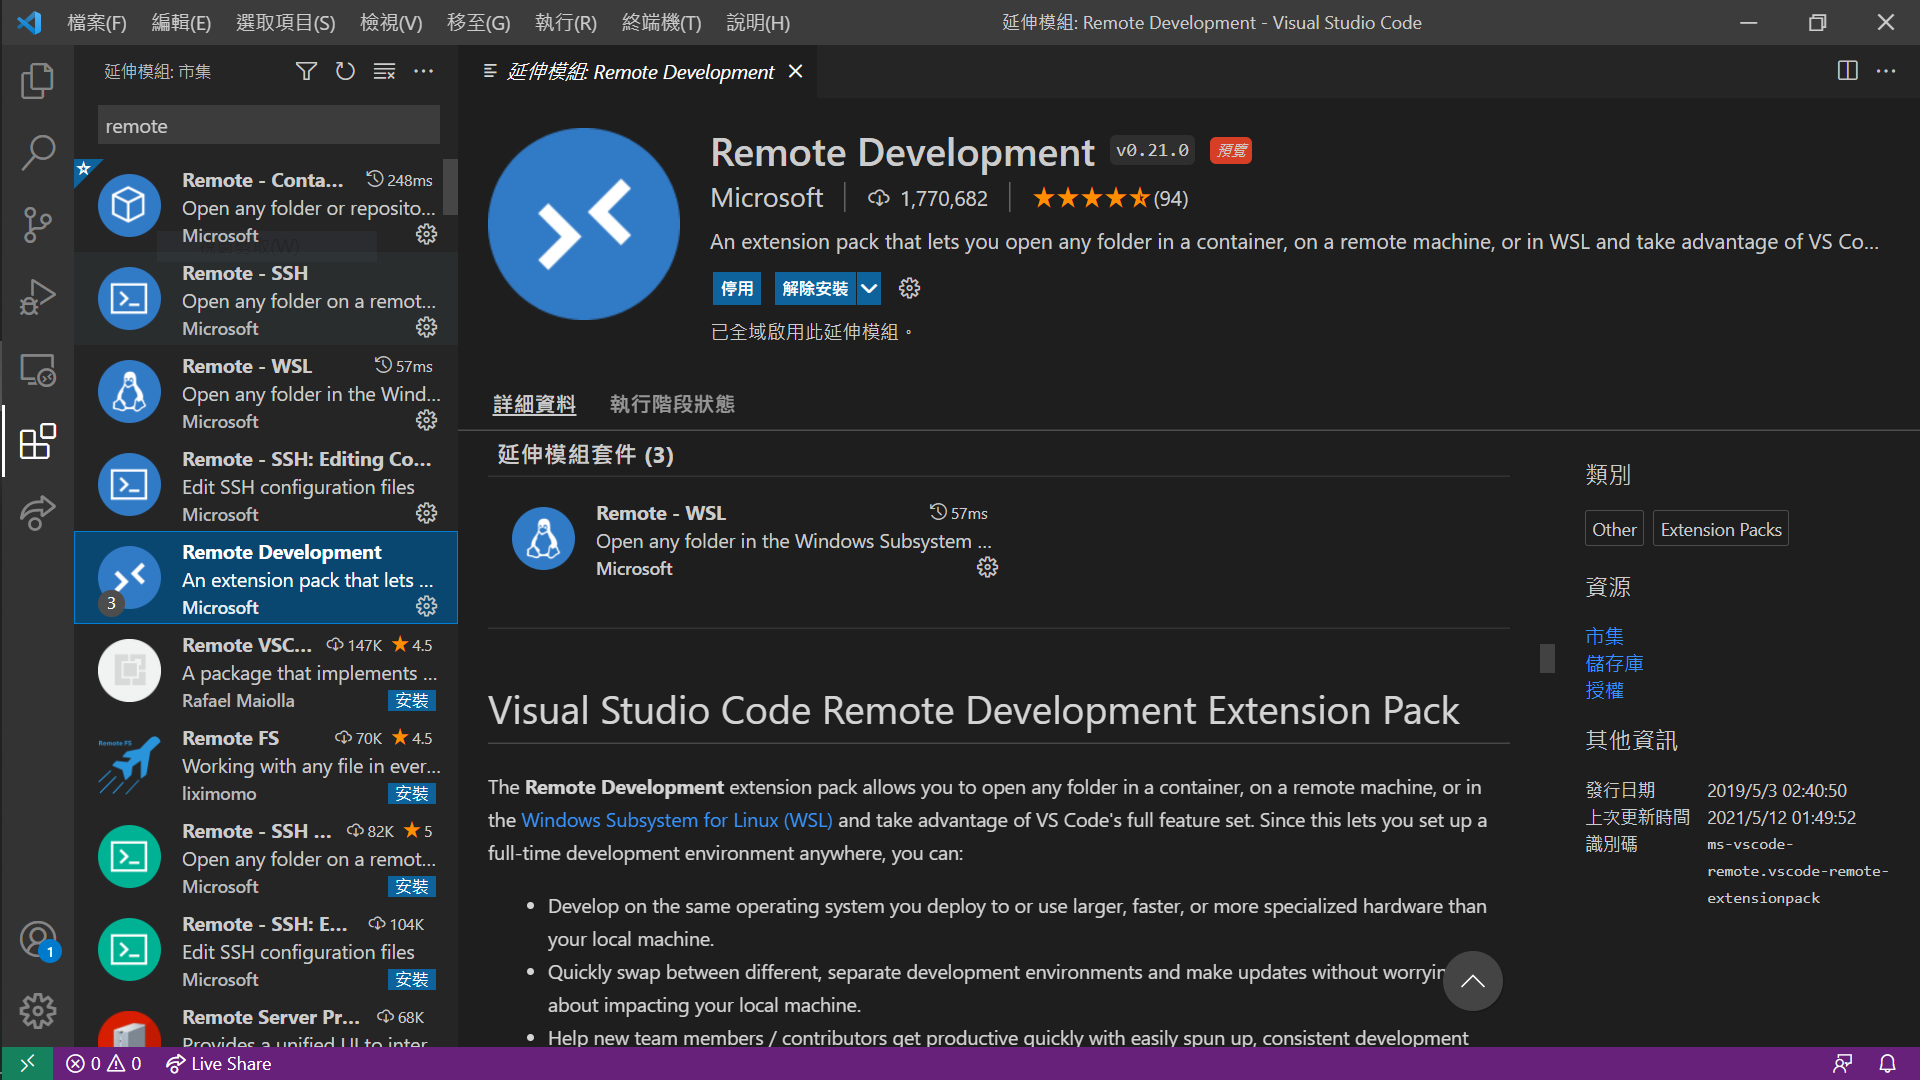
\includegraphics[width=0.8\textwidth]{./Figures/Env/docker/vscode_remote_extension.png} 
        \caption{安裝 remote extension}
        \label{fig_vscode_remote_extension}
\end{figure}

\subsubsection*{步驟三}

啟動 container 進行服務可雙擊檔案或以 terminal 於專案目錄中執行啟動指令。如果正常運作執行後終端機將會自動關閉。

\begin{flushleft}
        \textbf{Linux、MacOS、WSL}
\end{flushleft}

\begin{lstlisting}[language=bash]
        $ ./Docker/linux/start
\end{lstlisting}

\begin{flushleft}
        \textbf{Windows}
\end{flushleft}

\begin{lstlisting}[language=bash]
        > ./Docker/windows/start.bat
\end{lstlisting}

\subsubsection*{步驟四}

Ctrl-P 呼叫命令工具,找到(可直接輸入) \emph{> Remote-Container: Attach to Running container ...},如圖\ref{fig_vscode_select_container},點擊後選擇 latex-srv 即可進入開發環境,如圖\ref{fig_vscode_attach_container}。

\begin{figure}[H] 
        \centering 
        \subfigure{
                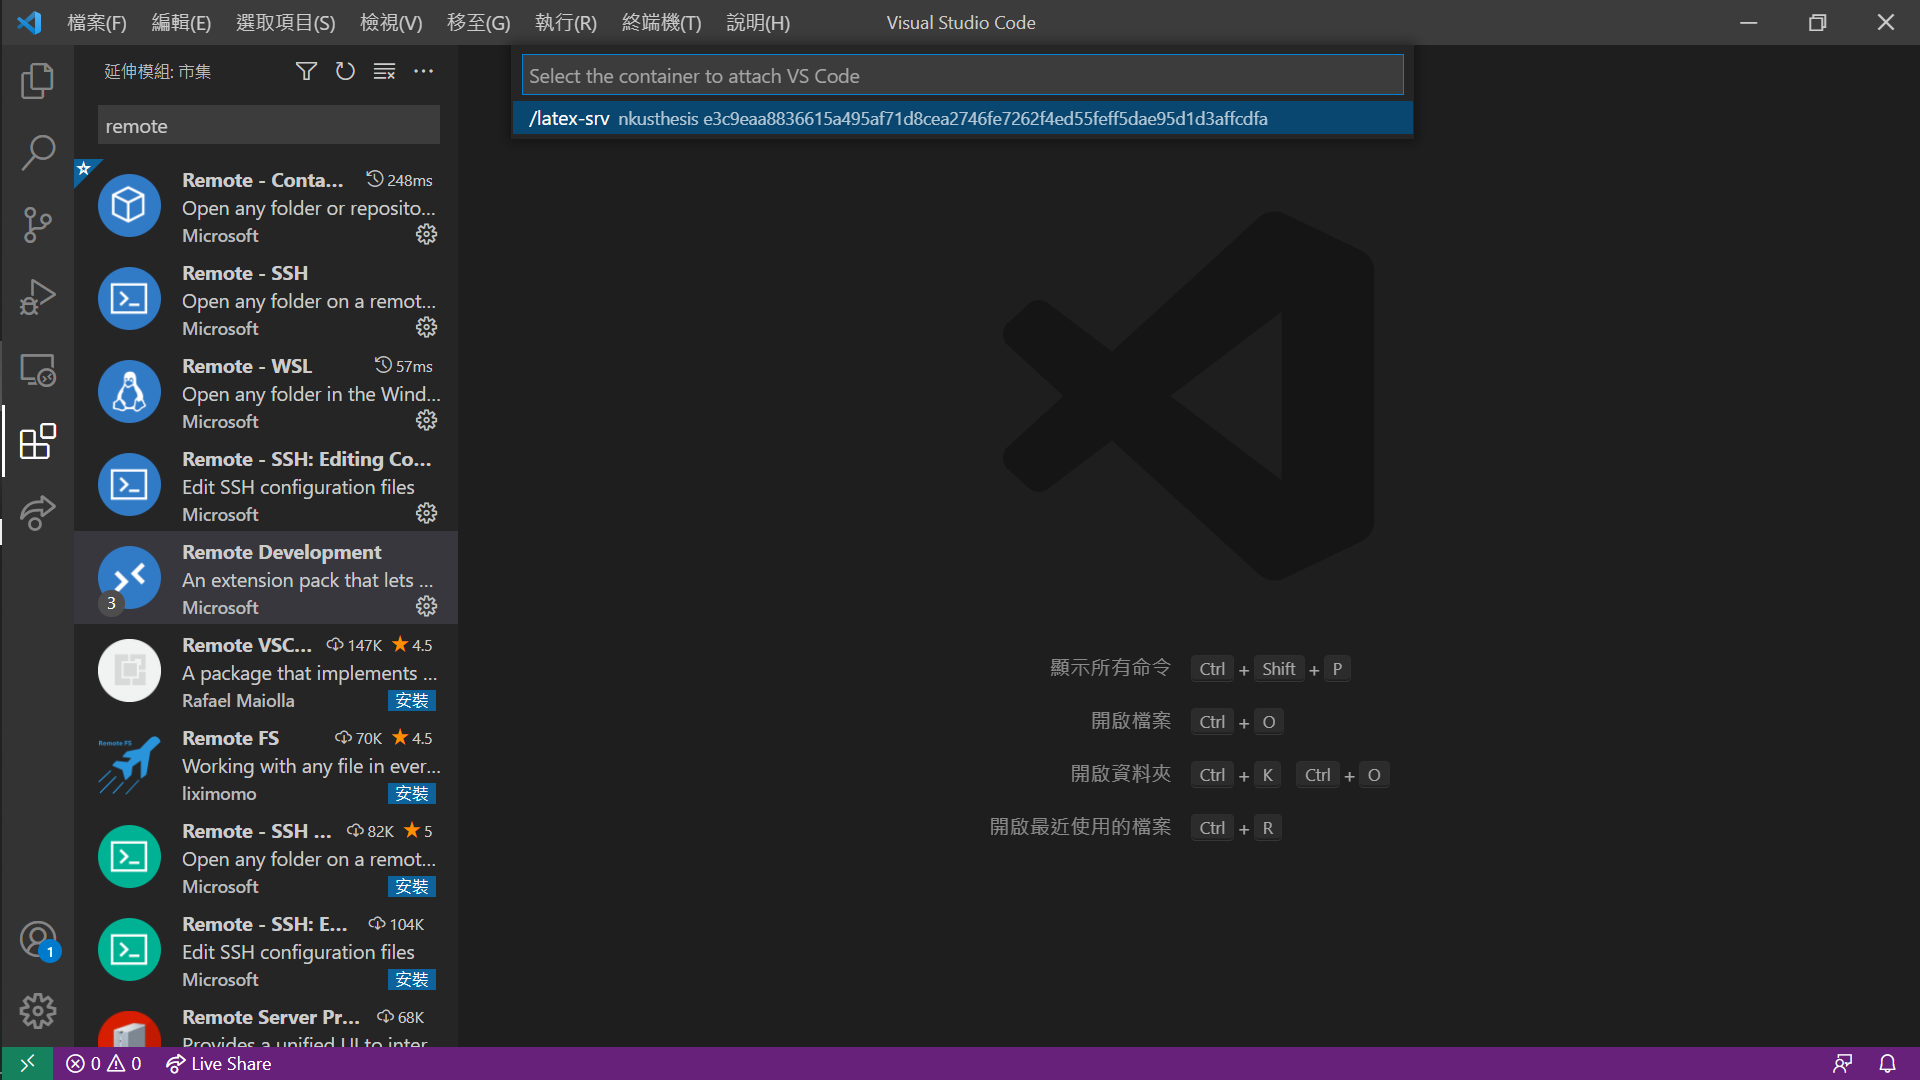
\includegraphics[width=0.8\textwidth]{./Figures/Env/docker/vscode_select_container.png}
                \label{fig_vscode_select_container}
        }
        \quad
        \centering 
        \subfigure{
                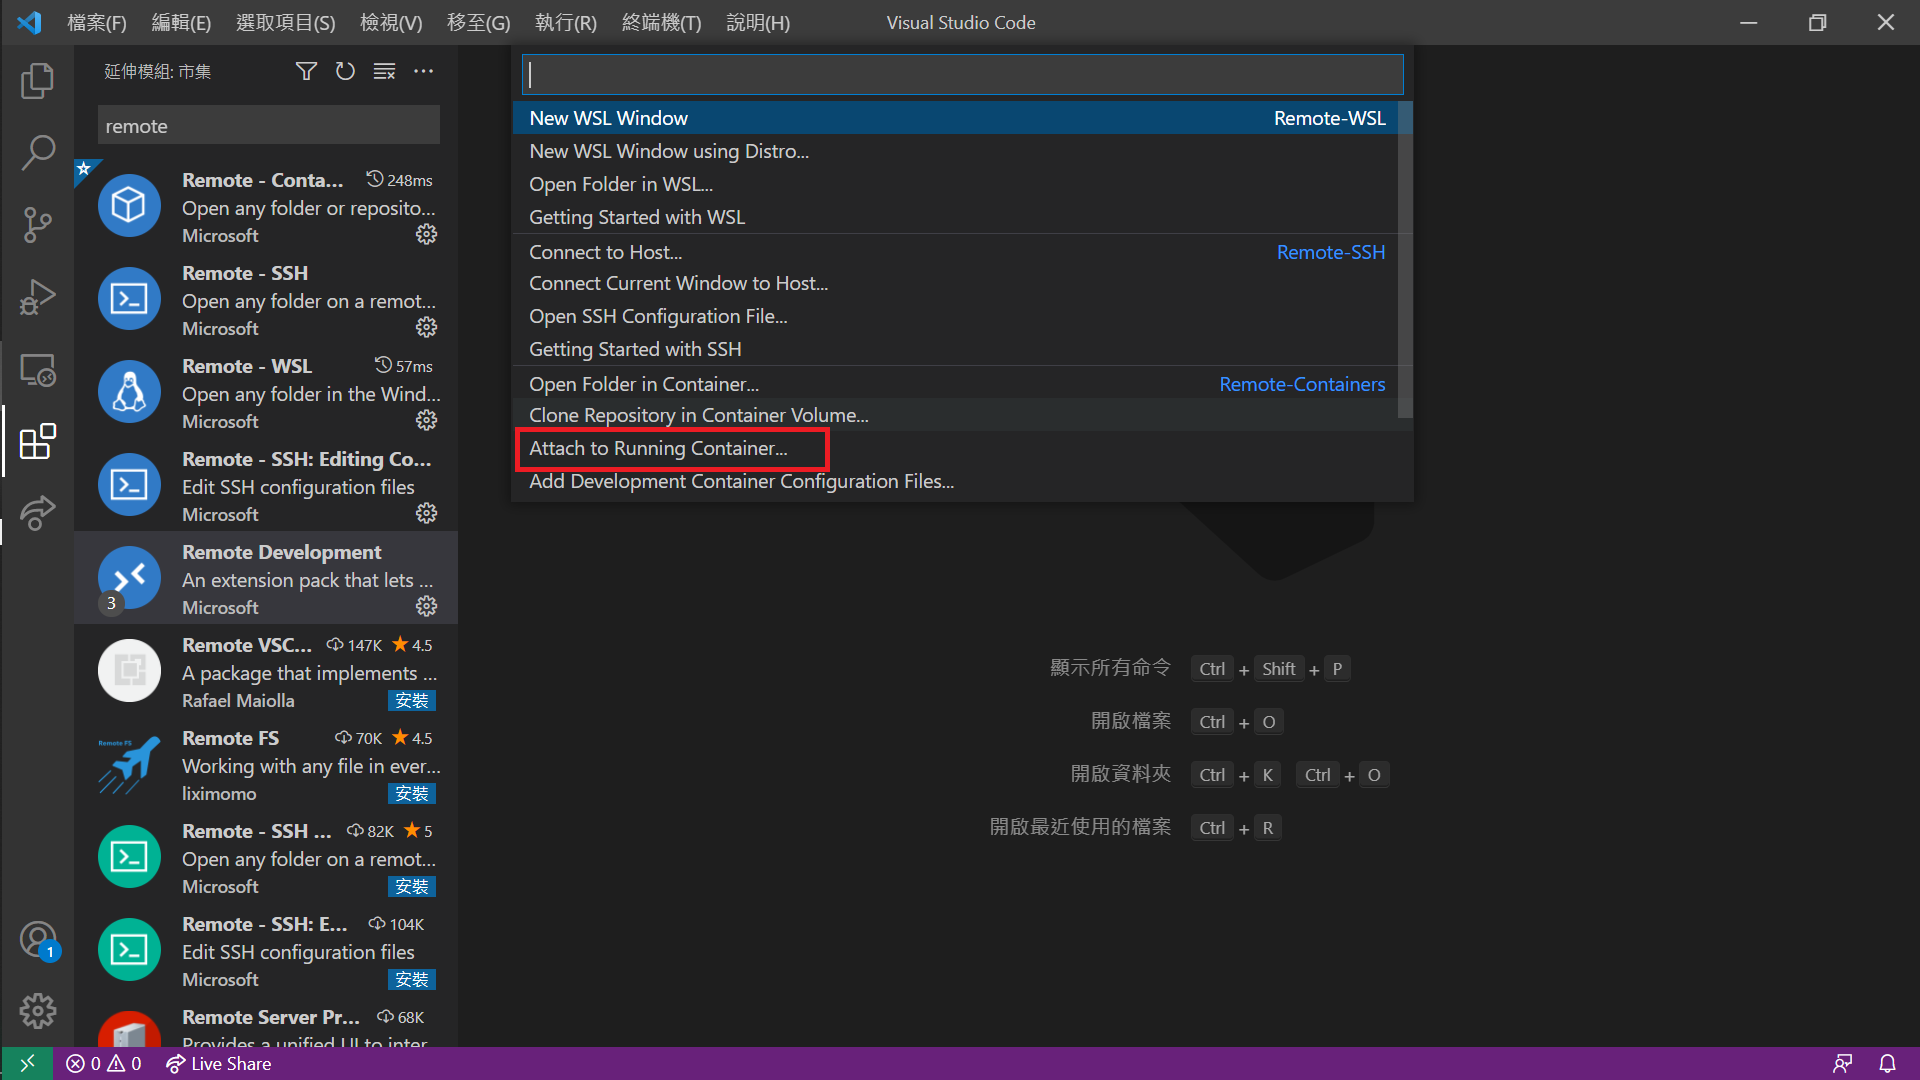
\includegraphics[width=0.8\textwidth]{./Figures/Env/docker/vscode_attach_container.png}
                \label{fig_vscode_attach_container}
        }
        \caption{Attach to Running container}
\end{figure}

\subsubsection*{步驟五}

開啟資料夾,論文目錄預設掛載在 \emph{/home/<username>/thesis} 中,如圖\ref{fig_vscode_finish}。

\begin{figure}[H] 
        \centering 
        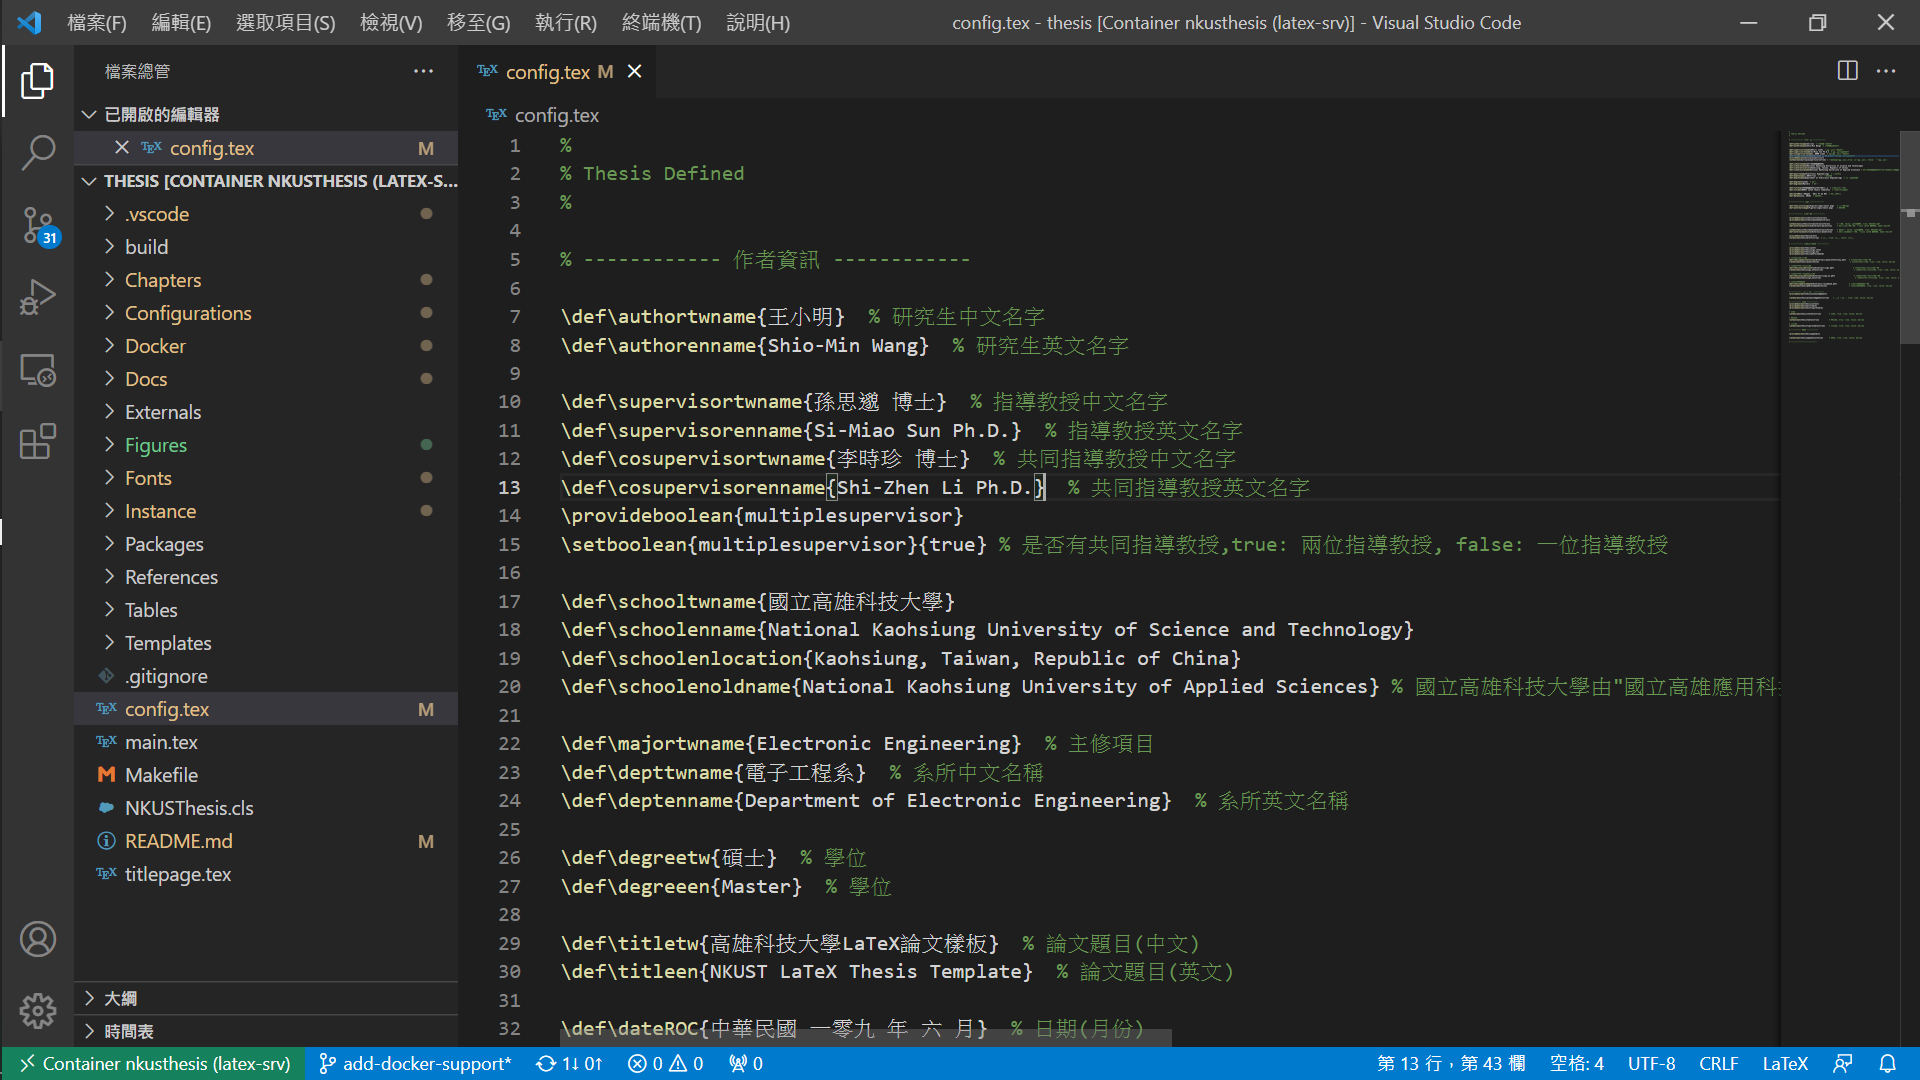
\includegraphics[width=0.8\textwidth]{./Figures/Env/docker/vscode_finish.png} 
        \caption{完成開啟 Container 中的論文目錄}
        \label{fig_vscode_finish}
\end{figure}

\chapter{版型設定} \label{ch_tmp_config}

本章內容包含論文資訊、論文Logo、封面、相關文件引入以及版型微調等。
章節內使用到的檔案有 config.tex、thesisinfo.tex 以及 Configurations 中的 tex 檔案。

\section{論文資訊}

論文作者、指導教授、學校等不變的訊息,其設定位於 thesisinfo.tex 中。
設定中如有碰到 zhtw、tw 或 en 表示這個項目有區分中英文的。

\begin{lstlisting}[language=TeX]
    \def\authortwname{王小明}
    \def\authorenname{Shio-Min Wang}
\end{lstlisting}

目前規範中有一個項目需特別注意,因本校是由三所科技大學合併而成,因此論文需加入原本所屬學校的英文名稱。
下方為原校英文名稱的欄位,請依原校英文名進行修改。

\begin{lstlisting}[language=TeX]
    \def\schoolenoldname{National Kaohsiung University of Applied Sciences}
\end{lstlisting}

此欄位在未來如果被取消,請發個 Issue 通知我們,謝謝!

\section{初稿與正式版}

給予口試委員的論文為初稿。因此需要封面加入初稿字樣,可透過 config.tex 進行設定。
當設定為 ture 時會產生初稿字樣,設定為 false 表示為正式版初稿字樣將會被隱藏。

\begin{lstlisting}[language=TeX]
    \setboolean{thesisdraft}{true}
    \setboolean{thesisdraft}{false}
\end{lstlisting}

\section{外部檔案匯入與啟用設定}

論文中的封面、書名頁皆可透過 LaTeX 產生,當您已經額外製作封面與書名頁時,可透過外部匯入的方式來取代。
另外博碩士論文授權書、論文口試委員會審定書、論文口試委員會英文審定書、博士論文推薦書皆由外部匯入,論文內無法自動產生。

\subsection*{封面}

封面要使用外部檔案時請將參數 isthesistitleexternal 設定為 true,
並將 externalmaintitle 參數導向至您放置 pdf 檔案的位置。

\begin{lstlisting}[language=TeX]
    \setboolean{isthesistitleexternal}{false}
    \def\externalmaintitle{Externals/maintitle}
\end{lstlisting}

\subsection*{書名頁}
書名頁與封面相同,預設為使用 LaTeX 產生,如需使用外部匯入,請修改 isthesisbooknameexternal 為 true,
並將 externalbooktitle 參數導向至您放置 pdf 檔案的位置。

\begin{lstlisting}[language=TeX]
    \setboolean{isthesisbooknameexternal}{false}
    \def\externalbooktitle{Externals/booktitle}
\end{lstlisting}

\subsection*{授權書與審定書}

授權書、審定書以及英文審定書皆由國家圖書館與學校提供,LaTeX 不提供此版型,因此需額外匯入,
請在匯入時注意修改的規範。載入請設定為 true,不載入請設定為 false。並依照該欄位說明填入指定的 pdf 檔案路徑。

碩博士論文授權書,由國家圖書館發布,依照規定正本應繳回圖書館,
此文件是否需放入論文中尚無定論,端看老師與系辦是否要求,
如需插入本頁文件,應當由您列印文件後簽署,再將簽署好的文件掃描插入此頁中。
\begin{lstlisting}[language=TeX]
    \def\thesispowerofattorney{Externals/powerofattorney.pdf}
    \setboolean{thesisauht}{false}
\end{lstlisting}

當您的論文口試委員審定書使用正本則請忽略此頁,如使用掃描檔案插入則請開啟此頁。
審定書有分中英文,故此將二個項目分開。此文件請由 https://acad.nkust.edu.tw/p/412-1004-2503.php?Lang=zh-tw 進行下載,
下載前建議您先確認本年度是否依然使用此份文件。

\begin{lstlisting}[language=TeX]
    \def\thesisvalidationzhtw{Externals/sign.pdf}
    \setboolean{thesissign_zhtw}{true}
    \def\thesisvalidationen{Externals/sign_en.pdf}
    \setboolean{thesissign_en}{true}
\end{lstlisting}

\subsection*{博士論文推薦書}
碩士不需要使用博士論文推薦書,此項目操作手法與審定書等相同。
\begin{lstlisting}[language=TeX]
    \def\thesisphdrecommand{Externals/recommand.pdf}
    \setboolean{thesisphdrecommand}{false}
\end{lstlisting}

\section{LaTeX 文件啟用與關閉}

\subsection*{誌謝與序言}

誌謝與序言在本專案中被視為相同的文件,載入該文件使用將 thesisacknowledgement 參數設為 true,反之則設為 false。
如您需要修改內容,請由 Instance/acknowledgement.tex 進行編輯。

\begin{lstlisting}[language=TeX]
    \setboolean{thesisacknowledgement}{true}
\end{lstlisting}

\subsection*{目錄列表}

論文中包含了 3 種目錄,文件目錄、圖目錄、表目錄,當您論文沒有使用到圖片或表格時,將會產生多餘的頁數,
因此提供使用者手動屏蔽該頁的功能,載入目錄使用 ture,屏蔽目錄則使用 false。

\begin{lstlisting}[language=TeX]
    \setboolean{thesiscontent}{true}
    \setboolean{thesistable}{true}
    \setboolean{thesisfiguretable}{true}
\end{lstlisting}

\subsection*{附錄}

附錄是論文的附加文件,在本專案的 3 個實驗室中,皆無附加附錄的功能。
因此此欄位預設為關閉狀態,如需啟用請自行在 Configurations/appendice.tex 中加入該附錄內容,如何修改此內容將於下一章節進行說明。

\begin{lstlisting}[language=TeX]
    \setboolean{thesisappendix}{false}
\end{lstlisting}

\chapter{如何開始撰寫自己的論文內容} \label{ch_how2start}

相信目前的文件數量仍然會讓您在評估上仍許多疑惑,
為了避免讓您在撰寫論文時遇到許多的小問題,本章將會一步步帶著您將本專案修改為您自己的論文。

\section{架構簡介}

本專案所有的設定都盡可能的模組化,讓每個目錄、檔案的操作內容皆能專注在特定的事務上。在開始之前先一一介紹本專案的架構。

\begin{itemize}
    \item Chapter - 論文各章節文件
    \item Configurations - 論文設定
    \item Docker - Docker 環境設定與執行檔
    \item Docs - 專案參考文件
    \item Externals - 外部匯入文件
    \item Figures - 圖片
    \item Fonts - 字體檔案
    \item Instance - 論文文章以外的文件
    \item Packages - LaTeX package
    \item References - 參考文獻
    \item Tables - 表格
    \item Templates - 版型 sty 檔案
\end{itemize}

需要由使用者自行新增 tex 文件的目錄有 Chapter、Externals、Figures、Tables、References,這些目錄都是放置論文內容的地方,
需要進行微調的目錄有 Configurations、Instance,其餘目錄則不建議變動。

\section{如何編輯}

\subsection*{Chapter 的新增、刪除、修改}

chapter 是存放內容文件的目錄,考慮到每個人的章節數量不同,因此章節載入及章節順序獨立於 Configurations/chapter.tex 中。
當然您也可以直接在一個文件中完成所有論文章節。

當您要加入一個章節,請先在 Chapters 中建立您的要新增的檔案(以下以 A.tex 作為範例)。
並在 Configurations/chapter.tex 加入這個檔案,讓編譯時被專案引入到檔案中。

\begin{lstlisting}[language=TeX]
    \input{Chapters/A.tex}
\end{lstlisting}

接著開始進行文件編輯,在邏輯上我們希望每個章節都存放在不同的 tex 檔案中,因此需要先定義此頁的章節名稱。
接著就可以開始進行論文撰寫了,如您需要更多的小節,可使用 section、subsection、subsubsection 來定義小節。

\begin{lstlisting}[language=TeX]
    \chapter{A.tex 範例01}\label{leb1}
    
    \section{小節1}
    
    \subsection{小節1-1}
    \subsection{小節1-2}
    \subsubsection{小節1-2-1}
    \subsubsection{小節1-2-2}
    \subsection{小節1-3}
    \section{小節2}
    \section{小節3}
\end{lstlisting}

當您不希望小節被加入到目錄,您可以使用 * 號來進行忽略目錄號碼。

\begin{lstlisting}[language=TeX]
    \subsection*{忽略小節號碼}
\end{lstlisting}

\subsection*{Externals、Figures、Tables}

Externals、Figures 是用來儲存匯入論文的文件、圖片用。Tables 是表格 tex 文件的儲存空間,如表格不大會建議直接將圖表直接放在 chapter 中。

匯入外部 PDF 檔案語法如下,IfFileExists 用於檢查檔案是否存在,檔案存在才會將該檔案進行引入。在編譯時引入一個不存在的檔案,將會造成編譯錯誤。
\begin{lstlisting}[language=TeX]
    \IfFileExists{Externals/ext.pdf}{
        \includepdf[pagecommand={\thispagestyle{empty}}]{Externals/ext.pdf}
    }{}
\end{lstlisting}

下方列出引入表格檔案的 tex 檔案,這個做法和加入 A.tex 到 chapter.tex 的行為相同。
\begin{lstlisting}[language=TeX]
    \input{Tables/a.tex}
\end{lstlisting}

\subsection*{Reference 修改}

本專案的 reference 工具是 bib,下面將介紹 IEEE xplore 網站的文件取得論文的 bib 的格式。

如圖\ref{fig_bib_1},在該篇論文網站的左上角,點下 Cite This 會出現如圖\ref{fig_bib_2}的視窗,切換至 BibTex 分頁即複製這份論文的 bib 語法。
再將段文字貼上到 References/reference.bib 中即可。

\begin{figure}[H] 
    \centering 
    \includegraphics[width=0.5\textwidth]{./Figures/how_to_used/ieee_xplore_cite_this_bib_01.png} 
    \caption{cite this}
    \label{fig_bib_1}
\end{figure}

\begin{figure}[H] 
    \centering 
    \includegraphics[width=0.5\textwidth]{./Figures/how_to_used/ieee_xplore_cite_this_bib_02.png} 
    \caption{bibtex text}
    \label{fig_bib_2}
\end{figure}

\input{Chapters/latex_example.tex}
\input{Chapters/algorithm.tex}
\input{Chapters/experimental_picture.tex}

\chapter{結論} \label{conclusion_and_future}

\section{命令總結}

\subsection*{產生論文}

經過開發者討論後,決議將論文與封面產生皆由 all 指令產生。

\begin{lstlisting}[language=bash]
    make all
\end{lstlisting}

\subsection*{清除暫存}

暫存檔案檔案是由 xelatex 編譯時所產生,使用此指令清除暫存並不會將 PDF 檔案清除。

\begin{lstlisting}[language=bash]
    make clean
\end{lstlisting}

\subsection*{完整清除}

完整清除檔案會將所有由 xelatex 編譯產生的檔案完整清除,包含論文與封面的 PDF 檔案。

\begin{lstlisting}[language=bash]
    make distclean
\end{lstlisting}

\subsection*{PDF防拷加工}

透過 ghostscript\cite{ghostscript} 為 PDF 提供防拷功能,其指令如下。

\begin{lstlisting}[language=bash]
    make pdfprocessing
\end{lstlisting}

此功能依賴 build/main.pdf 作為加工來源,因此當 build/main.pdf 不存在導致無法執行此命令時,請先執行 make all 來產生檔案。

\section{結語}

未來,我們也不知道能持續維護多久,只要有人使用,我們就會盡力維護下去。
目前僅支援 Linux,未來將會盡量朝向支援 Windows,讓更多人能使用此專案。

如果這個專案給您提供了幫助,請給我們 GitHub Repository\cite{github-repo} 一個 Star 讓我們知道。
最後祝福您順利畢業!

% ------------------


    }{}

    % 參考文獻
    \IfFileExists{Instance/reference}{
        \input{Instance/reference.tex}
    }{}

    % 附錄
    \IfFileExists{Configurations/appendice}{
        % 論文附錄的tex檔案載入請放置於 Configurations/appendice.tex 中
        \input{Configurations/appendice}
    }{}

    %----------------------------------------------------------------------------------------
    %	論文內容 結束
    %----------------------------------------------------------------------------------------

    % 自傳或簡歷 (可有可無)

    % 書背 (此欄為空)
    \newpage \thispagestyle{empty} \newpage

    %----------------------------------------------------------------------------------------

    \clearpage
\end{document}
